\documentclass[a4paper]{article}

%=========================================
% Packages
%=========================================
\usepackage{mathtools}
\usepackage{amsfonts}
\usepackage{amsmath}
\usepackage{amssymb}
\usepackage{amsthm}
\usepackage[a4paper, total={6in, 8in}, margin=1in]{geometry}
\usepackage[utf8]{inputenc}
\usepackage{fancyhdr}
\usepackage[utf8]{inputenc}
\usepackage{graphicx}
\usepackage{physics}
\usepackage[listings]{tcolorbox}
\usepackage{hyperref}
\usepackage{tikz-cd}
\usepackage{adjustbox}
\usepackage{enumitem}
\usepackage[font=small,labelfont=bf]{caption}
\usepackage{subcaption}
\usepackage{wrapfig}
\usepackage{makecell}



\raggedright

\usetikzlibrary{arrows.meta}

\DeclarePairedDelimiter\ceil{\lceil}{\rceil}
\DeclarePairedDelimiter\floor{\lfloor}{\rfloor}

%=========================================
% Fonts
%=========================================
\usepackage{tgpagella}
\usepackage[T1]{fontenc}


%=========================================
% Custom Math Operators
%=========================================
\DeclareMathOperator{\adj}{adj}
\DeclareMathOperator{\im}{im}
\DeclareMathOperator{\nullity}{nullity}
\DeclareMathOperator{\sign}{sign}
\DeclareMathOperator{\dom}{dom}
\DeclareMathOperator{\lcm}{lcm}
\DeclareMathOperator{\ran}{ran}
\DeclareMathOperator{\ext}{Ext}
\DeclareMathOperator{\dist}{dist}
\DeclareMathOperator{\diam}{diam}
\DeclareMathOperator{\aut}{Aut}
\DeclareMathOperator{\inn}{Inn}
\DeclareMathOperator{\syl}{Syl}
\DeclareMathOperator{\edo}{End}
\DeclareMathOperator{\cov}{Cov}
\DeclareMathOperator{\vari}{Var}
\DeclareMathOperator{\cha}{char}
\DeclareMathOperator{\Span}{span}
\DeclareMathOperator{\ord}{ord}
\DeclareMathOperator{\res}{res}
\DeclareMathOperator{\Hom}{Hom}
\DeclareMathOperator{\Mor}{Mor}
\DeclareMathOperator{\coker}{coker}
\DeclareMathOperator{\Obj}{Obj}
\DeclareMathOperator{\id}{id}
\DeclareMathOperator{\GL}{GL}
\DeclareMathOperator*{\colim}{colim}

%=========================================
% Custom Commands (Shortcuts)
%=========================================
\newcommand{\CP}{\mathbb{CP}}
\newcommand{\GG}{\mathbb{G}}
\newcommand{\F}{\mathbb{F}}
\newcommand{\N}{\mathbb{N}}
\newcommand{\Q}{\mathbb{Q}}
\newcommand{\R}{\mathbb{R}}
\newcommand{\C}{\mathbb{C}}
\newcommand{\E}{\mathbb{E}}
\newcommand{\Prj}{\mathbb{P}}
\newcommand{\RP}{\mathbb{RP}}
\newcommand{\T}{\mathbb{T}}
\newcommand{\Z}{\mathbb{Z}}
\newcommand{\A}{\mathbb{A}}
\renewcommand{\H}{\mathbb{H}}
\newcommand{\K}{\mathbb{K}}

\newcommand{\mA}{\mathcal{A}}
\newcommand{\mB}{\mathcal{B}}
\newcommand{\mC}{\mathcal{C}}
\newcommand{\mD}{\mathcal{D}}
\newcommand{\mE}{\mathcal{E}}
\newcommand{\mF}{\mathcal{F}}
\newcommand{\mG}{\mathcal{G}}
\newcommand{\mH}{\mathcal{H}}
\newcommand{\mI}{\mathcal{I}}
\newcommand{\mJ}{\mathcal{J}}
\newcommand{\mK}{\mathcal{K}}
\newcommand{\mL}{\mathcal{L}}
\newcommand{\mM}{\mathcal{M}}
\newcommand{\mO}{\mathcal{O}}
\newcommand{\mP}{\mathcal{P}}
\newcommand{\mS}{\mathcal{S}}
\newcommand{\mT}{\mathcal{T}}
\newcommand{\mV}{\mathcal{V}}
\newcommand{\mW}{\mathcal{W}}

%=========================================
% Colours!!!
%=========================================
\definecolor{LightBlue}{HTML}{2D64A6}
\definecolor{ForestGreen}{HTML}{4BA150}
\definecolor{DarkBlue}{HTML}{000080}
\definecolor{LightPurple}{HTML}{cc99ff}
\definecolor{LightOrange}{HTML}{ffc34d}
\definecolor{Buff}{HTML}{DDAE7E}
\definecolor{Sunset}{HTML}{F2C57C}
\definecolor{Wenge}{HTML}{584B53}
\definecolor{Coolgray}{HTML}{9098CB}
\definecolor{Lavender}{HTML}{D6E3F8}
\definecolor{Glaucous}{HTML}{828BC4}
\definecolor{Mauve}{HTML}{C7A8F0}
\definecolor{Darkred}{HTML}{880808}
\definecolor{Beaver}{HTML}{9A8873}
\definecolor{UltraViolet}{HTML}{52489C}



%=========================================
% Theorem Environment
%=========================================
\tcbuselibrary{listings, theorems, breakable, skins}

\newtcbtheorem[number within = subsection]{thm}{Theorem}%
{	colback=Buff!3, 
	colframe=Buff, 
	fonttitle=\bfseries, 
	breakable, 
	enhanced jigsaw, 
	halign=left
}{thm}

\newtcbtheorem[number within=subsection, use counter from=thm]{defn}{Definition}%
{  colback=cyan!1,
    colframe=cyan!50!black,
	fonttitle=\bfseries, breakable, 
	enhanced jigsaw, 
	halign=left
}{defn}

\newtcbtheorem[number within=subsection, use counter from=thm]{axm}{Axiom}%
{	colback=red!5, 
	colframe=Darkred, 
	fonttitle=\bfseries, 
	breakable, 
	enhanced jigsaw, 
	halign=left
}{axm}

\newtcbtheorem[number within=subsection, use counter from=thm]{prp}{Proposition}%
{	colback=LightBlue!3, 
	colframe=Glaucous, 
	fonttitle=\bfseries, 
	breakable, 
	enhanced jigsaw, 
	halign=left
}{prp}

\newtcbtheorem[number within=subsection, use counter from=thm]{lmm}{Lemma}%
{	colback=LightBlue!3, 
	colframe=LightBlue!60, 
	fonttitle=\bfseries, 
	breakable, 
	enhanced jigsaw, 
	halign=left
}{lmm}

\newtcbtheorem[number within=subsection, use counter from=thm]{crl}{Corollary}%
{	colback=LightBlue!3, 
	colframe=LightBlue!60, 
	fonttitle=\bfseries, 
	breakable, 
	enhanced jigsaw, 
	halign=left
}{crl}

\newtcbtheorem[number within=subsection, use counter from=thm]{eg}{Example}%
{	colback=Beaver!5, 
	colframe=Beaver, 
	fonttitle=\bfseries, 
	breakable, 
	enhanced jigsaw, 
	halign=left
}{eg}

\newtcbtheorem[number within=subsection, use counter from=thm]{ex}{Exercise}%
{	colback=Beaver!5, 
	colframe=Beaver, 
	fonttitle=\bfseries, 
	breakable, 
	enhanced jigsaw, 
	halign=left
}{ex}

\newtcbtheorem[number within=subsection, use counter from=thm]{alg}{Algorithm}%
{	colback=UltraViolet!5, 
	colframe=UltraViolet, 
	fonttitle=\bfseries, 
	breakable, 
	enhanced jigsaw, 
	halign=left
}{alg}




%=========================================
% Hyperlinks
%=========================================
\hypersetup{
    colorlinks=true, %set true if you want colored links
    linktoc=all,     %set to all if you want both sections and subsections linked
    linkcolor=DarkBlue,  %choose some color if you want links to stand out
}


\pagestyle{fancy}
\fancyhf{}
\rhead{Labix}
\lhead{Topological Manifolds}
\rfoot{\thepage}

\title{Topological Manifolds}

\author{Labix}

\date{\today}
\begin{document}
\maketitle
\begin{abstract}
\end{abstract}
\pagebreak
\tableofcontents
\pagebreak

\section{Topological Manifolds and Singular Homology}
\subsection{Covering Spaces of Manifolds}
\begin{prp}{}{} Any covering space of a manifold is also a manifold. 
\end{prp}

\subsection{Orientability}
Recall the notion of orientation in finite dimensional vector bases. We say that two bases of a vector space have the same orientation if the change of basis matrix has determinant greater than $0$. Since topological manifolds locally look like finite-dimensional vector spaces, we expect that orientations can be generalized to manifolds. \\~\\

The key observation in defining orientation through homology is the following proposition, which shows that the local homology groups on a manifold are isomorphic to $\Z$ on the top dimension. 

\begin{prp}{}{} Let $M$ be a $k$-dimensional topological manifold and $x\in M$ a point. Then $$H_n(M,M\setminus\{x\})\cong H_n(\R^k,\R^k\setminus\{\ast\})\cong\begin{cases}
\Z & \text{ if } n=k\\
0 & \text{ if } n\neq k
\end{cases}$$ \tcbline
\begin{proof}
Let $x\in U$ be an open neighbourhood such that $U\cong\R^k$. Then by excision, we have that $$H_n(M\setminus(M\setminus U),(M\setminus\{x\})\setminus(M\setminus U))\cong H_n(M,M\setminus\{x\})$$ This translates to $H_n(U,U\setminus\{x\})\cong H_n(\R^k,\R^k\setminus\ast)$. By corollary 5.2.3 in Algebraic Topology 2, we are done. Alternatively, we have the following proof: \\~\\

If $k=0$, the results are clear. If $k\geq 1$, then the long exact sequence of the pair $(\R^k,\R^k\setminus\ast)$ together with the fact that $\R^k\setminus\ast\simeq S^{k-1}$ and $\R^k\simeq\ast$ gives $$H_n(\R^k,\R^k\setminus\ast)=0$$ for $n>k$ and $n<k$. When $n=k$, we have an exact sequence \\~\\
\adjustbox{scale=1.0,center}{\begin{tikzcd}
	0 & {H_k(\R^k,\R^k\setminus\ast)} & {H_{k-1}(S^{k-1})} & {H_{k-1}(\R^k)}
	\arrow[from=1-1, to=1-2]
	\arrow[from=1-2, to=1-3]
	\arrow[from=1-3, to=1-4]
\end{tikzcd}}\\~\\
when $k>1$ since $H_{k-1}(\R^k)=0$. Thus $H_k(\R^k,\R^k\setminus\ast)\cong\Z$. If $k=1$, then the last map $H_0(S^0)\to H_0(\R)$ is given by the matrix $\begin{pmatrix}
1 & 1
\end{pmatrix}:\Z^2\to\Z$ thus also giving isomorphism. 
\end{proof}
\end{prp}

\begin{defn}{Local Orientation}{} A local orientation of $M$ at $x$ is a choice of generator of $H_k(M,M\setminus\{x\})$. 
\end{defn}

One can think of local orientation as follows. Choose an open neighbourhood $U$ of $x$ that is homeomorphic to $\R^2$. Then the long exact sequence for relative homology gives an isomorphism $$H_2(U,U\setminus\{x\})\cong H_1(S^1)$$ since $U\setminus\{x\}$ deformation retracts onto a small circle around $x$, we can choose a local orientation $\omega_x$ for the circle which is the same as choosing in which direction to loop around the circle. It remains to patch them up into a global orientation. Of course, this does not necessarily work for every single manifold. \\~\\

Let $U$ be a chart on a topological manifold $M$ and that $B\subseteq M$ is such that on the chart $U$, $B$ is an open / closed ball $B_r(z)$. For convention, we give a name to subsets of these type. 

\begin{defn}{Open and Closed Ball in Manifolds}{} Let $M$ be a $k$-dimensional topological manifold and $U$ a chart of $M$. We say that $B$ is an open / closed ball if under the homeomorphism of the chart $U\cong\R^k$, the image of $B$ is a ball $B_r(x)\subseteq\R^k$ for some $r\in\R^+$ and $x\in\R^k$. 
\end{defn}

The point of the definition is that we have the following sequence of isomorphisms 

\begin{align*}
H_k(M,M\setminus B)&\cong H_k(U,U\setminus B)\tag{Excise $M\setminus U$}\\
&\cong H_k(\R^k,\R^k\setminus B_r(x))
\end{align*}

and then using the long exact sequence in relative homology, we obtain an isomorphism $$H_k(\R^k,\R^k\setminus B_r(x))\cong H_{k-1}(\R^k\setminus B_r(x))$$ in which the latter space deformation retracts onto the boundary $\partial B_r(x)\cong S^{k-1}$. Thus $$H_k(\R^k,\R^k\setminus B_r(x))\cong H_{k-1}(\partial B_r(x))\cong\Z$$ is infinite cyclic. This means that we can think of the choice of a local orientation as a choice of orientation on $\partial B_r(x)$. \\~\\

Notice that the inclusion $(M,M\setminus B)\hookrightarrow(M,M\setminus\{y\})$ induces a map in homology: $$H_k(M,M\setminus B)\overset{\cong}{\rightarrow}H_k(M,M\setminus\{y\})$$ It is an isomorphism since $B$ is homeomorphic to a ball in $\R^k$ which is contractible. This leads to the following definition. 

\begin{defn}{Consistent Local Orientations}{} Let $(\omega_y)_{y\in B}$ be a family of local orientations. We say that it is consistent if there is a generator $\omega_B\in H_k(M,M\setminus B)$ such that $\omega_B\mapsto\omega_y$ for each $y\in B$ under the isomorphism $$H_k(M,M\setminus B)\cong H_k(M,M\setminus\{y\})$$
\end{defn}

With this, we can now formally define orientations in a manifold. 

\begin{defn}{Orientation of a Manifold}{} Let $M$ be a $k$-dimensional topological manifold. An orientation of $M$ is a function $$x\mapsto\omega_x\in H_k(M,M\setminus\{x\})$$ assigning every point to a local orientation such that for every $x\in M$, there exists an open ball $x\in B$ such that $(\omega_x)_{x\in B}$ a consistent local orientation. 
\end{defn}

Since $H_k(M,M\setminus\{x\})$ is isomorphic to $\Z$, this means that there are only two possible choices of distinct orientation classes for each point $x\in M$. 

\begin{lmm}{}{} The $k$-sphere $S^k$ is orientable for any $k\in\N$. \tcbline
\begin{proof}
Choose a fundamental class in $H_k(S^k)$. It is clear that the long exact sequence in relative homology induces a map $$H_k(S^k)\to H_k(S^k,S^k\setminus\{x\})$$ induces local orientation at each point $x\in S^k$. They are locally consistent since the map factors through $H_k(S^k,S^k\setminus B)$ for any open ball $B$ in $S^k$. 
\end{proof}
\end{lmm}

In order to deduce orientability of a manifolds, we appeal to a vector bundle on the manifold. 

\begin{defn}{Orientation Bundle}{} Let $M$ be a topological manifold. Define the orientation bundle $\widetilde{M}$ to be the set of pairs $$\widetilde{M}=\left\{(x,\omega_x)\;\bigg{|}\;\; x\in M, \omega_x\in H_k(M,M\setminus\{x\})\right\}$$ together the projection map $\pi:\widetilde{M}\to M$ defined by $\pi(x,\omega_x)=x$ and with the topology defined as follows. \\~\\

Let $B$ be an open ball in $M$. Since there are exactly two distinct orientation classes on $B$ we have that $$\pi^{-1}(B)=B_+\amalg B_-$$ where $B_+$ and $B_-$ are homeomorphic to $B$. Define the topology of $\widetilde{M}$ to be generated by sets of the form $B_+$ and $B_-$. 
\end{defn}

\begin{lmm}{}{} For any topological manifold $M$, $\widetilde{M}$ is a manifold and is a $2$-sheeted covering. \tcbline
\begin{proof}
Let $(x,\omega_x)$ and $(y,\omega_y)$ in $\widetilde{M}$ be distinct. If $x=y$ then $\omega_x=-\omega_y$. We know that there are two distinct orientation classes so $\pi^{-1}$ is a disjoint union consisting of those with positive orientation and those with negative. Since $\omega_x$ and $\omega_y$ are opposite, they lie in the disjoint union separately so that they are disjoint. If $x\neq y$, then since $M$ is Hausdorff then we can choose $U_1$ and $U_2$ disjoint neighbourhoods of $x$ and $y$ respectively. Then this means that $\pi^{-1}(U_1)$ and $\pi^{-1}(U_2)$ are disjoint. Thus we have shown that $M$ is Hausdorff. \\~\\

Now let $(x,\omega_x)\in\widetilde{M}$. Then since $M$ is manifold, there is an open ball $B$ around $x$ so that $B$ is homeomorphic to $\R^k$. $\pi^{-1}(B)$ is then a disjoint union of two copies of $B$, one such copy contains $(x,\omega_x)$. Then we have found a neighbourhood for $(x,\omega_x)$ that is homeomorphic to $\R^k$. Thus we are done. \\~\\

It is clear that it is a two sheeted covering because for any open set $B\subseteq M$, $\pi^{-1}(B)=B_+\amalg B_-$. 
\end{proof}
\end{lmm}

\begin{lmm}{}{} Let $M$ be a topological manifold. Then the orientation bundle $\widetilde{M}$ is orientable. \tcbline
\begin{proof}
To show orientability, it suffices to show that for every $(x,\omega_x)\in\tilde{M}$, there is a choice of orientation such that there exists an open set in $\tilde{M}$ for which the choice of orientation is locally consistent. So let $(x,\omega_x)$ be a point in $\tilde{M}$. Let $B$ be a small open ball around $x$ in $M$. Then $\pi^{-1}(B)$ is by definition a disjoint union of two copies of $B$, each with a locally consistent orientation. In other words, $\pi^{-1}(B)=A\amalg C$. Without loss of generality, take $(x,\omega_x)\in A$. Now consider the following isomorphisms $$H_k(\widetilde{M},\widetilde{M}\setminus\{(x,\omega_x)\})\cong H_k(A,A\setminus\{(x,\omega_x)\})\cong H_k(B,B\setminus\{x\})\cong H_k(M,M\setminus\{x\})$$ The first isomorphism is obtained by excising the piece $\widetilde{M}\setminus A$. The second isomorphism is obtained by considering the homeomorphism $\pi|_A$. The third isomorphism theorem is obtained by excising the piece $M\setminus B$ from the right. \\~\\

Thus for any choice of orientation in $H_k(M,M\setminus\{x\})$ we obtain a choice of orientation in $H_k(\widetilde{M},\widetilde{M}\setminus\{(x,\omega_x)\})$. 

By two more excisions, we obtain \\~\\
\adjustbox{scale=1.0,center}{\begin{tikzcd}
	{H_k(\widetilde{M},\widetilde{M}\setminus A)} && {H_k(\widetilde{M},\widetilde{M}\setminus\{(x,\omega_x)\})} \\
	\\
	{H_k(M,M\setminus B)} && {H_k(M,M\setminus\{x\})}
	\arrow["\cong", from=1-1, to=1-3]
	\arrow["\cong", from=3-1, to=3-3]
	\arrow["\cong"{description}, from=3-3, to=1-3]
\end{tikzcd}}\\~\\

Since $A$ is a locally consistent choice of orientations, there exists a generator $\omega_B\in H_k(M,M\setminus B)$ such that $\omega_B\mapsto\omega_x$ under the bottom map of the diagram. This $\omega_x$ then gives $\widetilde{\omega}_x\in H_k(\widetilde{M},\widetilde{M}\setminus\{(x,\omega_x)\})$. Which under the isomorphism of the top arrow in the diagram we obtain a generator of $H_k(\widetilde{M},\widetilde{M}\setminus A)$. Since each operation described is independent of the choice of $x\in B$, the generator we obtained for $H_k(\widetilde{M},\widetilde{M}\setminus A)$ is independent of the choice of $(x,\omega)_x$. Thus the consistent local orientation condition is satisfied so that $\widetilde{M}$ is orientable. 
\end{proof}
\end{lmm}

\begin{lmm}{}{} The deck transformation of the orientation bundle of manifold is orientation reversing. \tcbline
\begin{proof}
Any non-trivial deck transformation must permute the fibers of the covering space non-trivially. In this case, any $(x,\omega_x)$ can only be mapped to the other of the element of the fiber which is $(x,-\omega_x)$. 
\end{proof}
\end{lmm}

\begin{lmm}{}{} Giving an orientation of $M$ is equivalent to giving a continuous map $s:M\to\widetilde{M}$ such that $s\circ\pi=\text{id}$ (section of the orientation bundle). \tcbline
\begin{proof}
Let $s:M\to\widetilde{M}$ be continuous and that $s\circ\pi=\text{id}$. Then $s$ assigns a orientation $\omega_x$ to each $x\in M$. The map is continuous if and only if for each open ball in $M$ and $\pi^{-1}(B)=B_+\amalg B_-$, the preimages $s^{-1}(B_+)$ and $s^{-1}(B_-)$ are both open in $B$. Since these two preimages are disjoint and jointly cover $B$, this condition is equivalent $s(B)=B_+$ or $s(B)=B_-$. This precisely means that the local orientations are consistent. 
\end{proof}
\end{lmm}

\begin{thm}{}{} Let $M$ be a connected topological manifold. Then exactly one of the following holds: 
\begin{itemize}
\item $\widetilde{M}\to M$ is a non-trivial $2$-sheeted cover and $M$ is non-orientable
\item $\widetilde{M}\cong M\amalg M$ and $M$ admits precisely two orientations
\end{itemize} \tcbline
\begin{proof}
Assume that $\pi:\widetilde{M}\to M$ is connected and $\omega:M\to\widetilde{M}$ is a continuous section to $\pi$. Let $x\in M$ and $\pi^{-1}(x)=\{(x,\omega_x),(x,-\omega_x)\}$. By assumption there is a path $\gamma$ in $\widetilde{M}$ from $(x,\omega_x)$ to $(x,-\omega_x)$. Then $\gamma$ and $\omega\circ\pi\circ\gamma$ are two paths in $\widetilde{M}$ lifting $\pi\circ\gamma$ and starting at $(x,\omega_x)$. But the first path ends at $(x,-\omega_x)$ and the second one ends at $(x,\omega_x)$. This is a contradiction to the uniqueness of lifting paths. Thus $M$ is non-orientable. \\~\\

If $M$ is disconnected then $\widetilde{M}\cong M\amalg M$ since $\widetilde{M}$ is a covering space. Thus $M$ admits two orientations. 
\end{proof}
\end{thm}

\begin{crl}{}{} Any simply connected manifold is orientable. \tcbline
\begin{proof}
By Galois theory of covering spaces, any $2$-sheeted cover of a simply connected space is disconnected. 
\end{proof}
\end{crl}

\begin{prp}{}{} Let $k\geq 1$. Then $\R\Prj^k$ is orientable if and only if $k$ is odd. \tcbline
\begin{proof}
The quotient map $q:S^k\to\R\Prj^k$ is the unique connected two-sheeted cover of $\R\Prj^k$ by Galois theory for covering spaces. The non-trivial deck transformation is given by the antipodal map which has degree $(-1)^{k+1}$. If $k$ is odd then this degree is $1$ so that the deck transformation is orientation preserving. Since deck transformations of the orientation bundle must be orientation reversing, we conclude that $S^k\neq\widetilde{\R\Prj^k}$. This means that the orientation bundle of $\R\Prj^k$ is disconnected. \\~\\

Now assume that $k$ is even. By the lifting criterion, there exists a lift of $q$ called $\tilde{q}$ such that \\~\\
\adjustbox{scale=1.0,center}{\begin{tikzcd}
	& {\widetilde{\R\Prj^k}} \\
	{S^k} & {\R\Prj^k}
	\arrow["p", from=1-2, to=2-2]
	\arrow["{\tilde{q}}", from=2-1, to=1-2]
	\arrow["q", from=2-1, to=2-2]
\end{tikzcd}}\\~\\
where $p$ is the covering map. Then $\tilde{q}$ must also be a covering space. Assume that $q$ is not injective. This means that $\tilde{q}\circ(-\text{id})=\tilde{q}$ since $-\text{id}$ is the only other deck transformation of $S^k$ over $\R\Prj^k$. This means that for any $x\in S^k$, we have that \\~\\
\adjustbox{scale=1.0,center}{\begin{tikzcd}
	{H_k(S^k)} & {H_k(\widetilde{\R\Prj^k})} & {H_k(\widetilde{\R\Prj^k},\widetilde{\R\Prj^k}\setminus\{\tilde{q}(x)\})}
	\arrow["{\tilde{q}}", from=1-1, to=1-2]
	\arrow[from=1-2, to=1-3]
\end{tikzcd}}\\~\\
where the second map is given by the long exact sequence in relative homology. Denoting this entire map by $\alpha$, we have that $\alpha\circ(-\text{id})_\ast=\alpha$ since $\tilde{q}\circ(-\text{id})=\tilde{q}$. But $\alpha$ is a map from $\Z$ to $\Z$. Since $\alpha\circ(-\text{id})_\ast=\alpha$ this implies that $\alpha=0$. But $\alpha$ also factors as \\~\\
\adjustbox{scale=1.0,center}{\begin{tikzcd}
	{H_k(S^k)} & {H_k(S^k,S^k\setminus\{x\})} & {H_k(\widetilde{\R\Prj^k},\widetilde{\R\Prj^k}\setminus\{\tilde{q}(x)\})}
	\arrow["{\cong}", from=1-1, to=1-2]
	\arrow["{\tilde{q}}", from=1-2, to=1-3]
\end{tikzcd}}\\~\\
by the long exact sequence in relative homology and naturality. But the second map is also an isomorphism since covering spaces of manifolds induces a an isomorphism in local homology groups. \\~\\

Now $S^k$ being compact and $\R\Prj^k$ being Hausdorff together with $\tilde{q}$ being injective implies that $\tilde{q}$ is a homeomorphism onto an open and closed subspace of $\R\Prj^k$. Assume that $\tilde{q}$ is not surjective, then we have that $\widetilde{\R\Prj^k}\cong S^k\amalg X$ for some other space $X$. But this is impossible thus $q$ is surjective and $\tilde{q}$ gives a homeomorphism between $S^k$ and $\widetilde{\R\Prj^k}$. Since $S^k$ is connected, $\R\Prj^k$ is thus non orientable. 
\end{proof}
\end{prp}

One has to be careful that homotopy equivalence does not preserve orientability. For example, the Mobius strip is homotopy equivalent to $S^1$ but the former is non-orientable while the latter is. 

\subsection{Fundamental Class}
\begin{prp}{}{} Let $M$ be a connected compact smooth manifold of dimension $n$. If $M$ is orientable then $H_n(M)\cong\Z$. Otherwise $H_n(M)=0$. 
\end{prp}

\begin{defn}{Fundamental Class}{} Let $M$ be a connected compact orientable smooth manifold of dimension $n$. A fundamental class for $M$ is a generator for the top homology $$H_n(M)\cong\Z$$
\end{defn}

\pagebreak
\section{The Theory of Surfaces}
\subsection{Classification of Compact Surfaces}
Recall that a compact surface is a connected topological manifold of dimension $2$ that is compact. 

\begin{defn}{Connected Sum}{} Let $S_1$ and $S_2$ be two compact surfaces. Let $D_i\subseteq S_i$ be two small closed disks for $i=1,2$. Define the connected sum to be $$S_1\# S_2=\frac{(S_1\setminus D_1^\circ)\amalg(S_2\setminus D_2^\circ)}{\partial D_1\cong\partial D_2}$$
\end{defn}

\begin{lmm}{}{} The connected sum of two compact surfaces is again a surface. 
\end{lmm}

\begin{prp}{}{} The connected sum is invariant under the choice of homeomorphism and the location of the small discs. 
\end{prp}

We encounter our first family of compact surfaces by repeatedly applying connected sums to a number of toruses. 

\begin{defn}{$g$-Holed Torus}{} For $g\geq 0$, define the $g$-holed torus to be $$\Sigma_g=\T\#\cdots\#\T$$ the connected sum of $g$ toruses. By convention when $g=0$, $\Sigma_g$ is the $2$-sphere. 
\end{defn}

Recall the CW complex of the torus. We can visualize the connected sum of two toruses using the CW complex. 

\begin{center}
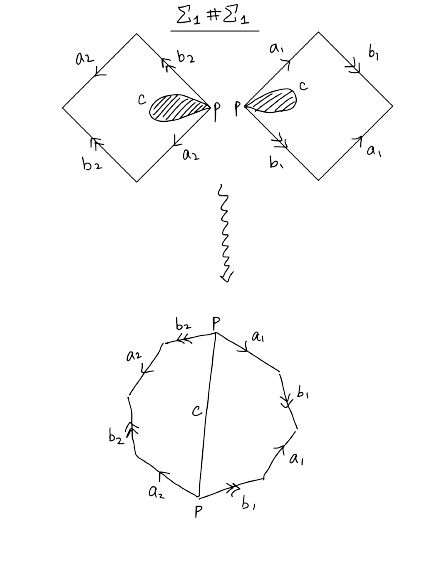
\includegraphics[scale = 0.8]{Image 1}
\end{center}

This is done by cutting a hole at the CW complex at the point $p$, and the pushing the boundary $c$ out, and then connecting them together. The cut-out hole is exactly a disc in the torus. By gluing the two toruses along the boundary $c$, we are effectively gluing the two toruses along the discs. \\~\\

The new hectagon obtained is precisely then the CW complex of $\Sigma_2$. In general, we can perform the operation of connected sum on a $(4g-4)$-gon and a square. We then obtain the CW complex of the $g$-holed torus. 

\begin{center}
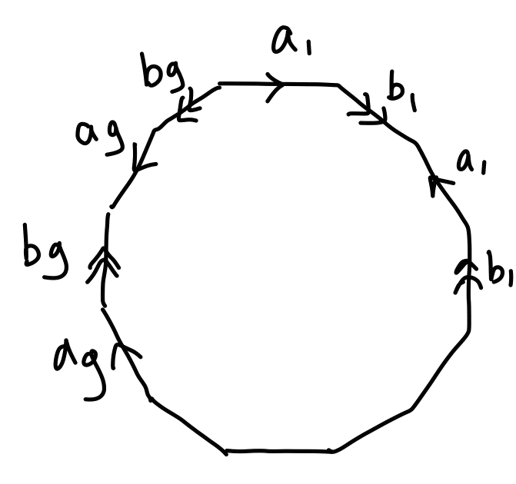
\includegraphics[scale = 0.3]{Image 2}
\end{center}

Another class of compact surfaces is the connected sum of projective spaces $\R\Prj^2$. 

\begin{defn}{Non-Orientable Surface}{} For $h\geq 1$, define $$N_h=\R\Prj^2\#\cdots\#\R\Prj^2$$ the connected sum of $h$ projective spaces. 
\end{defn}

We can do the same process of gluing the CW complexes just like that of the torus to obtain the $4h$-gon that represents $N_h$: 

\begin{center}
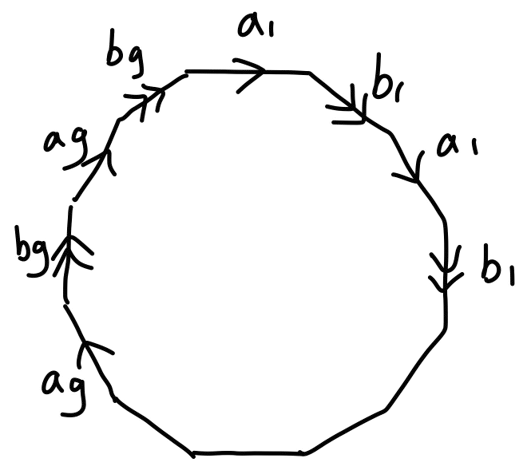
\includegraphics[scale = 0.3]{Image 3}
\end{center}

It is also meaningful to ask what would happen if we perform connected sums through the two class of compact surfaces. We obtain the following. 

\begin{prp}{}{} Let $N_3$ denote the connected sum of three projective spaces $\R\Prj^2$. Then we have that $$T\#\R\Prj^2=N_3$$ 
\end{prp}

The above two classes of compact surfaces together with the sphere exhausts all possible cases for compact surfaces. 

\begin{thm}{}{} Every compact surface is homeomorphic to exactly one of the following. 
\begin{itemize}
\item $\Sigma_g$ for $g\geq 0$
\item $N_h$ for $h\geq 1$
\end{itemize}
\end{thm}

\subsection{The Homology of Surfaces}
Recall that a compact surface is a connected topological manifold of dimension $2$ that is compact. Moreover, every compact surface is homeomorphic to either $\Sigma_g=\T\#\cdots\#\T$ for $g\geq 0$ or $N_h=\R\Prj^2\#\cdots\#\R\Prj^2$ for $h\geq 1$. We can now compute the homology groups of these surfaces and moreover, show that $\sum_g$ is orientable while $N_h$ is not, using the CW complexes given above. 

\begin{thm}{}{} Let $g\geq 0$. The homology of the $g$-holed torus $\Sigma_g$ is given by $$H_n(\Sigma_g)=\begin{cases}
\Z & \text{ if } n=0,2\\
\Z^{2g} & \text{ if } n=1\\
0 & \text{otherwise}
\end{cases}$$ \tcbline
\begin{proof}
Cut an open disc along the middle of the CW complex as follows

\begin{center}
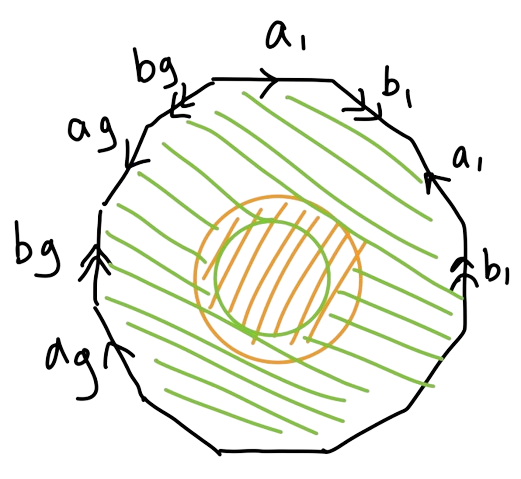
\includegraphics[scale = 0.3]{Image 4}
\end{center}

and label it $V$ (the orange part). Label the green part as $U$. It is clear that $U\cap V\simeq S^1$, $U$ is contractible and $V$ deformation retracts to the boundary, which is actually just a wedge sum of $2g$ circles. By the formula for the homology of wedge sums we have that $$H_n(V)=\begin{cases}
\Z & \text{ if } n=0\\
\Z^{2g} & \text{ if } n=1\\
0 & \text{ otherwise }
\end{cases}$$ By the reduced Mayer-Vietoris sequence, the only non-trivial homology groups in the sequence are \\~\\
\adjustbox{scale=1.0,center}{\begin{tikzcd}
	0 & {\tilde{H}_2(\Sigma_g)} & \Z & {\Z^{2g}} & {\tilde{H}_1(\Sigma_g)} & 0
	\arrow[from=1-1, to=1-2]
	\arrow[from=1-2, to=1-3]
	\arrow[from=1-3, to=1-4]
	\arrow[from=1-4, to=1-5]
	\arrow[from=1-5, to=1-6]
\end{tikzcd}}\\~\\
and the exact sequence \\~\\
\adjustbox{scale=1.0,center}{\begin{tikzcd}
	0 & {\tilde{H}_0(\Sigma_g)} & 0
	\arrow[from=1-1, to=1-2]
	\arrow[from=1-2, to=1-3]
\end{tikzcd}}\\~\\
in which the latter immediately shows that $H_0(\Sigma_g)\cong\Z$. Now the map $\Z\to\Z^{2g}$ sends a generator of the first homology of $U\cap V\simeq S^1$ to the loop $$a_1+b_1-a_1-b_1+\cdots+a_g+b_g-a_g-b_g$$ Since $\Z^{2g}$ is abelian, we conclude that this map is actually the zero map. It follows that $H_2(\Sigma_g)\cong\Z$ and $H_1(\Sigma_g)\cong\Z^{2g}$. 
\end{proof}
\end{thm}

We can immediate deduce the orientability of $\Sigma_g$ using the machinery in section $1$. 

\begin{crl}{}{} The surfaces $\Sigma_g$ for $g\geq 0$ is orientable. \tcbline
\begin{proof}
By the above, we have that $H_2(\Sigma_g)\cong\Z$. The long exact sequence for relative homology groups give \\~\\
\adjustbox{scale=0.9,center}{\begin{tikzcd}
	\cdots & {H_2(\Sigma_g\setminus\{x\})} & {H_2(\Sigma_g)} & {H_2(\Sigma_g,\Sigma_g\setminus\{x\})} & {H_1(\Sigma_g\setminus\{x\})} & {H_1(\Sigma_g)} & \cdots
	\arrow[from=1-1, to=1-2]
	\arrow[from=1-2, to=1-3]
	\arrow[from=1-3, to=1-4]
	\arrow[from=1-4, to=1-5]
	\arrow[from=1-5, to=1-6]
	\arrow[from=1-6, to=1-7]
\end{tikzcd}}\\~\\
Let $U$ be as the proof above. Then the inclusion from $U$ to $\Sigma\setminus\{x\}$ is a homotopy equivalence. Moreover, $\Sigma\setminus\{x\}$ is a $2g$-fold wedge of circles labelled $a_1,b_1,\dots,a_g,b_g$ and $H_2(\Sigma_g\setminus\{x\})=0$. Also, we have that $H_1(U)\cong H_1(\Sigma_g)$ from above and hence $H_1(\Sigma_g\setminus\{x\})\cong H_1(\Sigma_g)$. The last map is invertible so that by exactness, the third map is the zero map. Then what remains is an isomorphism $$H_2(\Sigma_g)\cong H_2(\Sigma_g,\Sigma_g\setminus\{x\})$$ Now since this isomorphism factors through $H_2(\Sigma_g,\Sigma_g\setminus B)$ for any ball $B$ containing $x$, we thus have a consistent local orientation throughout all of $\Sigma_g$. 
\end{proof}
\end{crl}

\begin{thm}{}{} Let $h\geq 1$. The homology of $N_h$ is given by $$H_n(N_h)=\begin{cases}
\Z & \text{ if } n=0\\
\Z^{h-1}\oplus\Z/2\Z & \text{ if } n=1\\
0 & \text{otherwise}
\end{cases}$$ \tcbline
\begin{proof}
Similar to the proof in that of $\Sigma_g$, cut an open disc along the middle of the CW complex of $N_h$ as follows 

\begin{center}
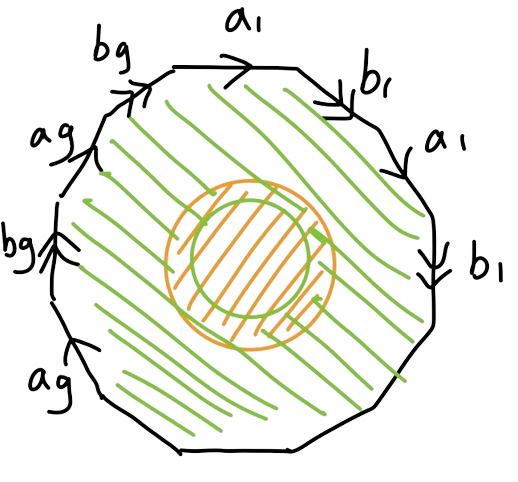
\includegraphics[scale = 0.3]{Image 5}
\end{center}

and again label the green part $U$ and the orange part $V$. Then apply Mayer-Vietoris sequence to acquire a similar exact sequence \\~\\
\adjustbox{scale=1.0,center}{\begin{tikzcd}
	0 & {\tilde{H}_2(\Sigma_g)} & \Z & {\Z^h} & {\tilde{H}_1(\Sigma_g)} & 0
	\arrow[from=1-1, to=1-2]
	\arrow[from=1-2, to=1-3]
	\arrow[from=1-3, to=1-4]
	\arrow[from=1-4, to=1-5]
	\arrow[from=1-5, to=1-6]
\end{tikzcd}}\\~\\
together with $\tilde{H}_0(N_h)\cong 0$. Notice that the third non-zero term counting from the left is now $\Z^h$ instead of $\Z^{2g}$ as in the torus because the boundary circle is the wedge sum of $h$ circles labelled $a_1b_1,\dots,a_hb_h$. The map $\Z$ to $\Z^h$ is now given by sending the generator $1$ to $$2(a_1+b_1+\dots+a_h+b_h)$$ The Smith Normal form of the matrix is an $h\times 1$ matrix with $2$ at the first entry and $0$ everywhere else. In particular, it means that this map is injective so that $\tilde{H}_2(N_h)\to\Z$ is the $0$ map so that $\tilde{H}_2(N_h)\cong 0$. Now it remains an exact sequence \\~\\
\adjustbox{scale=1.0,center}{\begin{tikzcd}
	0 & \Z & {\Z^h} & {\tilde{H}_1(N_h)} & 0
	\arrow[from=1-1, to=1-2]
	\arrow[from=1-2, to=1-3]
	\arrow[from=1-3, to=1-4]
	\arrow[from=1-4, to=1-5]
\end{tikzcd}}\\~\\
The image of the matrix is $2\Z$ and by exactness this is the kernel of the map $\Z^h\to\tilde{H}_1(N_h)$. Thus we have an isomorphism $$\tilde{H}_1(N_h)\cong\Z^{h-1}\oplus\Z/2\Z$$ and so we conclude. 
\end{proof}
\end{thm}

\begin{crl}{}{} The surfaces $N_h$ for $h\geq 1$ is non-orientable. \tcbline
\begin{proof}
Notice that removing a small closed disk from $\R\Prj^2$ yields a space homeomorphic to the open Mobius strip. It follows that for $h>0$, the space $N_h$ contains the open Mobius strip as a subspace. Since the Mobius strip is non-orientable, $N_h$ is also non-orientable. 
\end{proof}
\end{crl}

\subsection{The Euler Characteristic}
Recall that if $X$ is a CW complex such that $U\cap V=X$ and $U$ and $V$ are open subsets, then we have the formula $$\chi(X)=\chi(U)+\chi(V)-\chi(U\cap V)$$

\begin{crl}{}{} Let $S_1\# S_2$ be the connected sum of two compact surfaces, then we have that $$\chi(S_1\# S_2)=\chi(S_1)+\chi(S_2)-2$$ \tcbline
\begin{proof}
Let $D_i$ be the gluing discs for $S_i$ for $i=1,2$. Using the above formula, we have that $$\chi(S_i)=\chi(D_i)+\chi(S_i\setminus D_i^\circ)-\chi(S^1)$$ since the intersection of the disc and $S_i$ is $S^1$. It follows that 
\begin{align*}
\chi(S_1\# S_2)&=\chi(S_1\setminus D_1^\circ)+\chi(S_2\setminus D_2^\circ)-\chi(S^1)\\
&=\chi(S_1)+\chi(S_2)-2
\end{align*}
and so we conclude. 
\end{proof}
\end{crl}

\begin{crl}{}{} For $g\geq 0$ and $h>1$, the Euler characteristic of any compact surface is given by $$\chi(\Sigma_g)=2-2g\;\;\;\;\text{ and }\;\;\;\;\chi(N_h)=2-h$$ \tcbline
\begin{proof}
It follows directly by repeated applications of the above corollary. 
\end{proof}
\end{crl}

Recall that if $p:\tilde{X}\to X$ is a $d$-sheeted covering and $X$ is a finite CW complex, then we have the formula $$\chi(\tilde{X})=d\cdot\chi(X)$$


\pagebreak
\section{Cohomology on Manifolds}
\subsection{de Rham Cohomology}
\begin{prp}{}{} Let $M$ be a smooth manifold. Then differential forms of $M$, $\Omega^0(M),\dots,\Omega^n(M),\dots$ together with the exterior derivative $d:\Omega^n(M)\to\Omega^{n+1}(M)$ form a cochain complex. 
\end{prp}

\begin{defn}{}{} Let $M$ be a smooth manifold. Define the de Rham cohomology groups of $M$ to be the cohomology of the chain of differential forms: $$H_{\text{dR}}^n(M;\R)=H^n(\Omega^\bullet(M);\R)$$
\end{defn}

\begin{prp}{}{} Let $M$ be a smooth manifold of dimension $n$. Then the following are true for the de Rham cohomology of $M$. 
\begin{itemize}
\item $H_{\text{dR}}^k(M;\R)$ is a vector space over $\R$ for all $k\in\N$. 
\item For $r>n$ we have $H_{\text{dR}}^r(M;\R)=0$
\item If $M$ has $m$ connected components then $H_{\text{dR}}^0(M;\R)=\R^k$
\end{itemize}
\end{prp}

\begin{thm}{}{} Let $M$ be a smooth manifold of dimension $n$. Then the direct sum $$H^\ast(M)=\bigoplus_{k=1}^nH_{\text{dR}}^k(M;\R)$$ is an $\R$-algebra where multiplication defined by $a\wedge b\in H_{\text{dR}}^{s+l}(M;\R)$ for $a\in H_{\text{dR}}^s(M;\R)$ and $b\in H_{\text{dR}}^l(M;\R)$. Moreover, this multiplication is anti-commutative, namely for $a\in H_{\text{dR}}^s(M;\R)$ and $b\in H_{\text{dR}}^l(M;\R)$, we have $$a\wedge b=(-1)^{sl}b\wedge a$$
\end{thm}

\begin{prp}{}{} Let $M,N$ be smooth manifolds and $f:M\to N$ a smooth map. Then $f$ induces an $\R$-linear map $$f^\ast:H^\ast(N)\to H^\ast(M)$$ such that $f^\ast(a\wedge b)=f^\ast(a)\wedge f^\ast(b)$. Moreover, it is functorial: 
\begin{itemize}
\item If $g:N\to K$ is another smooth map of manifolds, then $(g\circ f)^\ast=f^\ast\circ g^\ast$
\item If $\text{id}:M\to M$ is the identity map on the manifold, then $\text{id}^\ast:H^\ast(M)\to H^\ast(M)$ is the trivial map on $\R$-algebras. 
\end{itemize}
\end{prp}

\begin{thm}{Homotopy Invariance of de Rham Cohomology}{} Let $f:M\times I\to N$ be a smooth map of manifolds varying for each $t\in I=[0,1]$. Write $f_t(x)=f(x,t)$. Then the pull back maps $f_0^\ast,f_1^\ast:H^\ast(N)\to H^\ast(M)$ are equal: $$f_0^\ast=f_1^\ast$$
\end{thm}

\subsection{de Rham Cohomology of Common Manifolds}
\begin{prp}{}{} The real space $\R^n$ has the de Rham cohomology $$H_{\text{dR}}^k(\R^n)=\begin{cases}
\R & \text{ if }k=0\\
0 & \text{ otherwise }
\end{cases}$$
\end{prp}

\begin{prp}{}{} The $n$-sphere $S^n$ has the de Rham cohomology $$H_{\text{dR}}^k(S^n)=\begin{cases}
\R & \text{ if }k=0,n\\
0 & \text{ otherwise }
\end{cases}$$
\end{prp}

\begin{thm}{}{} Let $p,q\geq 1$, the sphere $S^{p+q}$ is not diffeomorphic to any $M\times N$ manifolds where $\dim(M)=p$ and $\dim(N)=q$. 
\end{thm}

\begin{prp}{}{} Every smooth vector fields on $S^{2n}$ vanishes at some point of the sphere. 
\end{prp}

\begin{prp}{}{} The real projective space $\R\Prj^n$ has the de Rham cohomology $$H_{\text{dR}}^k(\R\Prj^n)=\begin{cases}
\R & \text{ if }k=0\text{ or }k=n\text{ where }n\text{ odd }\\
0 & \text{ otherwise }
\end{cases}$$
\end{prp}

\pagebreak
\section{Poincare Duality}
\subsection{The Cap Product}
\begin{defn}{The Cap Product}{} Let $\sigma=[v_0,\dots,v_k]\in C_k(X)$ and $\phi\in C^l(X)$ where $k\geq l$ with coefficients in a ring $R$. Define the cap product to be $$\sigma\frown\phi=\phi(\sigma|_{[v_0,\dots,v_l]})\sigma|_{[v_l,\dots,v_k]}\in C_{k-l}(X)$$
\end{defn}

\begin{lmm}{}{} The cap product $\frown: C_k(X)\times C^l(X)\to C_{k-l}(X)$ with coefficients in a ring $R$ induces a cap product in homology $\frown: H_k(X)\times H^l(X,R)\to H_{k-l}(X)$ for $k\geq l$. 
\end{lmm}

\subsection{Cohomology with Compact Support}

\subsection{The Duality Theorem}
\begin{thm}{Poincare Duality}{} Let $M$ be a compact and oriented topological $n$-manifold. Then the homomorphism $$D:H^p(M)\to H_{n-p}(M)$$ is an isomorphism. 
\end{thm}
















\end{document}
